\documentclass{article}

\usepackage{times}
\usepackage{amssymb, amsmath, amsthm}
\usepackage[margin=1in]{geometry}
\usepackage{graphicx}

\begin{document}

\title{MTH 351 HW 5}
\author{Philip Warton}
\date{\today}
\maketitle

\section*{1.}
Consider the function $f(x) = \dfrac{1}{4}(5-x^2)$.
\subsection*{a.}
We want to solve for all fixed points of $f$. We wish to find all $x$ where $f(x) = x$. We have, \[ \dfrac{1}{4}(5-x^2) = x. \] By arithmatic rearangement this is equivalent to the equation \[ 0 = x^2 +4x -5. \] Thus, we can factor the right hand side giving us, \[ 0 = (x-1)(x+5) \] This gives us solutions at $x = 1$ and $x = -5$.
\subsection*{b.}
For an iterative formula, we write \[ \dfrac{1}{4}(5-{x_n}^2) = {x_{n+1}}. \] With $x_0 = 0.8$,  we can plug this into our iterative formula on a calculator, which gives us $lim(x_n) = 1$. 
\subsection*{c.}
To verify this, let $L = lim(x_n) = lim(x_{n+1})$. Then,
\[ \dfrac{1}{4}(5-{L}^2) = {L} \] By arithmetic from \fbox{1a.}, we have $L = 1$ and $L = -5$.

% attach da picture

\subsection*{d.}
To find the order of convergence, let $e_{n} = | x_n - \alpha |$ and $e_{n+1} = | x_{n+1} - \alpha |$. Subtracting 1 from both sides of our iterative formula, we have 
\begin{align*}
 x_{n+1} - 1 & = \dfrac{1}{4}(5-x_n^2) -1 \\
e_{n+1} & = \dfrac{-1}{4}(x_n^2-1) \\
& = \dfrac{-1}{4}(e_n^2 - 2x_n) \ \ \ \ \ \ \ \ \ \ \ \ \ \ \ \ \ \ \ \text{(for large enough $n, x = 1$ thus)}\\
e_{n+1}& = \dfrac{2-e_n^2}{4}
\end{align*}
And we have an order of convergence of 2 for $f$.
\section*{2.}
\subsection*{a.}
\begin{figure}[h!]
	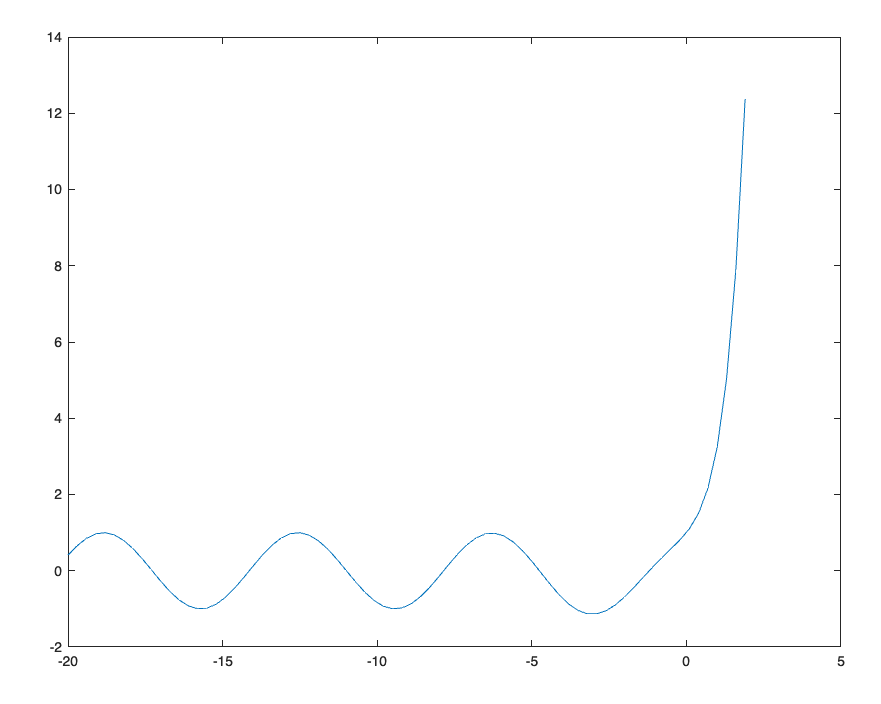
\includegraphics[scale=.3]{hw_5_matplot_graph_2}\
\end{figure}
\subsection*{b.}
To find the largest root for $f(x) = xe^x+cos(x)$ using Newton's method, let $x_0 = 0$. We know that $f'(x) = xe^x + e^x -sin(x)$. So our iteration method is 
\[ x_{n+1} = x_ne^{x_n}+cos(x_n) - \dfrac{x_ne^{x_n}+cos(x_n)}{x_ne^{x_n}+e^{x_n}-sin(x_n)}\]
The iteration will stop when $|x_n-x_{n+1}| < 10^{-4}$.
Using the online Geogebra app for Newton's root-finding method, we get that after 3 iterations we can stop, with the largest root being approximately at $x = -1.20106$.
\subsection*{c.}
To convert this problem to a fixed-point problem, we must begin with the equation that has solutions at every root,
\begin{align*}
0 &= xe^x + cos(x)\\
-x & = xe^x + cos(x) -x\\
x & = x-xe^x -cos(x)
\end{align*}
Now we have a fixed point problem with solutions at the roots of $f$. We have the iteration formula 
\[ x_{n+1} = x_n-x_ne^{x_n}-cos(x_n) \]
Let $x_0 = 0$, and we will stop iteration when $|x_n - x_{n+1}| < 10^{-4}$. After 6 iterations, we get the largest root to be at $x = -1.2011$, and there may be rounding due to my use of the Geogebra cobweb diagram applet.
\section*{3.}
Let $f(x) = x^2$.
\subsection*{a.} See hand-drawn paper attached
\subsection*{b.}
	For the iteration formula of Newton's method, we have $x_{n+1} = x_n + \dfrac{f(x)}{f'(x)}$. We can write \[x_{n+1} = x_n + \dfrac{x_n^2}{2x_n} \]
\subsection*{c.}
To find the limit of $x_n$, let $L = lim(x_n) = lim(x_{n+1})$. Then we have
\begin{align*}
	L & = L - \dfrac{L^2}{L} \\
	& = L - L\\
	&= 0
\end{align*}
For the order of convergence, let $e_{n+1} = x_{n+1} - 0$ and $e_n = x_n - 0$. Then,
 \begin{align*}x_{n+1} & = x_n + \dfrac{x_n^2}{2x_n} \\
e_{n+1} &= x_n + \dfrac{x_n}{2} \\
& =\dfrac{x_n}{2} \\
& = \dfrac{e_n}{2} \end{align*} Thus, we have a linear order of convergence with a rate of $\dfrac{1}{2}$.

\section*{4.} Find a polynomial passing through$(-1,1),(0,-1),(1,0),(2,2)$, denoted by $(x_1,y_1),( x_2,y_2),( x_3,y_3),( x_4,y_4)$. \subsection*{a.} Let $L_1(x) = \dfrac{(x-0)(x-1)(x-2)}{(-1)(-2)(-3)} = \dfrac{x^3-3x^2+2x}{-6}$, and let $L_2(x) = \dfrac{(x+1)(x-1)(x-2)}{(1)(-1)(-2)} = \dfrac{x^3-2x^2 - x+2}{2}$. Then let $L_3(x)=\dfrac{(x+1)(x)(x-2)}{(2)(1)(-1)} = \dfrac{x^3-x^2-2x}{-2}$. Finally, let $L_4(x)=\dfrac{(x+1)(x)(x-1)}{(3)(2)(1)} = \dfrac{x^3-x}{6}$. Then we have \[ P(x) = y_1 L_1(x) + y_2 L_2(x) + y_3 L_3 (x) + y_4 L_4(x)\] Given that we know $y_1, y_2, y_3, y_4$ and $L_1(x), L_2(x), L_3(x), L_4(x)$, we have \[ P(x) = (1) \dfrac{x^3-3x^2+2x}{-6} + (-1) \dfrac{x^3-2x^2 - x+2}{2} + (0) \dfrac{x^3-x^2-2x}{-2} + (2) \dfrac{x^3-x}{6}\] This can be simplified to \[P(x) = \dfrac{-1}{3}x^3+\dfrac{3}{2}x^2-\dfrac{1}{6}x-1\]

\subsection*{b.}
\begin{figure}[h!]
	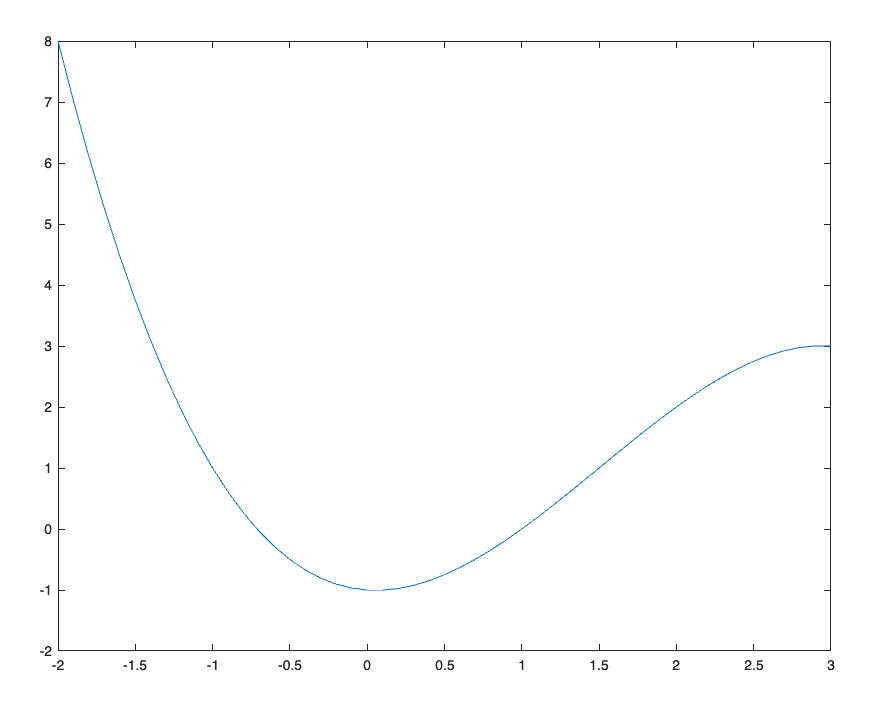
\includegraphics[scale=.3]{hw_5_matplot_graph}
\end{figure}
	% matlab plot need to do!!!

\subsection*{c.} Let $x = 1.5$. Then $P(1.5) = \dfrac{-1}{3}\left(\dfrac{27}{8}\right) + \dfrac{3}{2}\left(\dfrac{9}{4}\right) - \dfrac{1}{6}\left(\dfrac{3}{2}\right) - 1 $, which, when simplified, equals 1. For the slope at 1.5, write
	\[ P'(x) = -x^2 + 3x -\dfrac{1}{6}\] Then we have \[ P'(1.5) = -\dfrac{9}{4} + \dfrac{9}{2} - \dfrac{1}{6} = \dfrac{25}{12}\]




\end{document}